% Approximating a continuous function on [a,b] by a rectangle function
% whose rectangles have their upper-left corner on the graph.
% Source: book/tex/calculus/integrate.tex (§ Defining the Riemann integral).
\documentclass[border=2mm]{standalone}
\usepackage{tikz}
\begin{document}
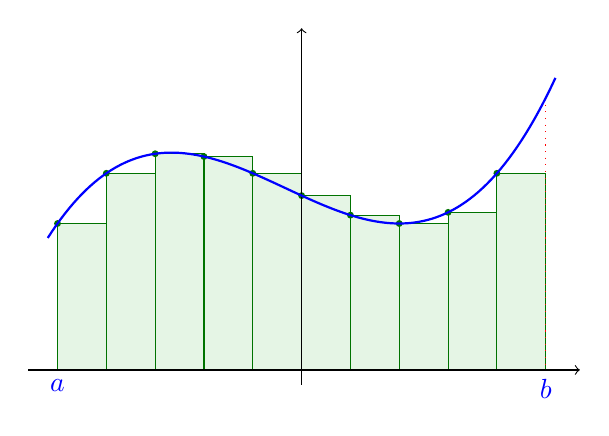
\begin{tikzpicture}[scale=0.62]
  \foreach \i in {0,...,9} {
    \pgfmathsetmacro\lx{\i-5}
    \pgfmathsetmacro\h{3+(\lx-2)*(\lx-2)*(\lx+5)/35}
    \fill[green!60!black,opacity=0.1] (\lx,0) rectangle (\lx+1,\h);
    \draw[green!45!black] (\lx,0) rectangle (\lx+1,\h);
    \fill[green!45!black] (\lx,\h) circle (2pt);
  }
  \draw[red,dotted] (5,{3+9*10/35})--(5,0);
  \draw[->] (-5.6,0)--(5.7,0);
  \draw[->] (0,-0.3)--(0,7);
  \draw[blue,thick,domain=-5.2:5.2,samples=120]
    plot (\x, {3+(\x-2)*(\x-2)*(\x+5)/35});
  \node[blue,below] at (-5,0) {$a$};
  \node[blue,below] at (5,0) {$b$};
\end{tikzpicture}
\end{document}
